\paragraph{QuizziPedia::Back-End::App::Controllers::QuestionController}
\label{QuizziPedia::Back-End::App::Controllers::QuestionController}
\begin{figure}[ht]
	\centering
	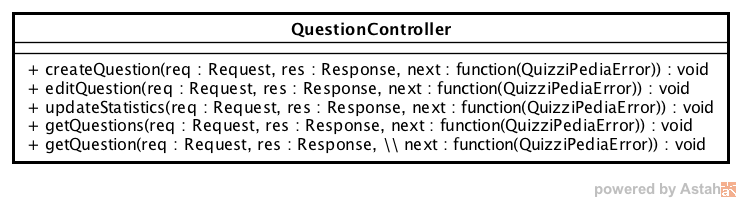
\includegraphics[scale=0.45]{UML/Classi/Back-End/QuizziPedia_Back-End_App_Controllers_questionController.png}
	\caption{QuizziPedia::Back-End::App::Models::Controllers::QuestionController}
\end{figure}
\FloatBarrier
	\begin{itemize}
		\item \textbf{Descrizione} \\
		Classe che gestisce la logica applicativa riguardante la visualizzazione, la creazione e la modifica delle domande presenti nell'applicazione;
		\item \textbf{Utilizzo} \\
		Viene utilizzata per implementare le funzionalità necessarie a gestire le richieste REST\ped{G} legate alle domande;
		\item \textbf{Relazioni con altre classi}
			\begin{itemize}
				\item \textbf{OUT \texttt{QuestionModel}} \\
				Classe che modella le domande dell'applicazione;
				\item \textbf{IN \texttt{QuestionRouter}} \\
				Classe che gestisce le richieste relative alle operazioni riguardanti le domande.
			\end{itemize}
		\item \textbf{Metodi}
			\begin{itemize}
				\item \texttt{+ createQuestion(req: Request, res: Response,\\ next: function(QuizziPediaError))} \\
				Crea e aggiunge una nuova domanda nel sistema. \\
				\textbf{Parametri:}
				\begin{itemize}
					\item \texttt{req: Request} \\
					Rappresenta la richiesta inviata al \textit{server\ped{G}}. Contiene l'identificativo dell'utente autenticato;
					\item \texttt{res: Response} \\
					Rappresenta la risposta che il \textit{server\ped{G}} fornirà al termine dell'esecuzione del metodo;
					\item \texttt{next: function(QuizziPediaError)} \\
					Rappresenta la \textit{callback\ped{G}} che il metodo deve chiamare al termine dell'elaborazione per passare il controllo ai successivi \textit{middleware\ped{G}}. La presenza del parametro facoltativo \texttt{QuizziPediaError} attiva la catena di gestione dell'errore in sostituzione della normale catena di gestione delle richieste.
				\end{itemize}
				\item \texttt{+ editQuestion(req: Request, res: Response,\\ next: function(QuizziPediaError))} \\
				Modifica una domanda già esistente nel sistema; \\
				\textbf{Parametri:}
					\begin{itemize}
						\item \texttt{req: Request} \\
						Rappresenta la richiesta inviata al \textit{server\ped{G}}. Contiene l'identificativo dell'utente autenticato. In \texttt{req} è presente un campo che rappresenta l'identificativo della domanda nel database che il metodo deve modificare e le relative modifiche;
						\item \texttt{res: Response} \\
						Rappresenta la risposta che il \textit{server\ped{G}} fornirà al termine dell'esecuzione del metodo;
						\item \texttt{next: function(QuizziPediaError)} \\
						Rappresenta la \textit{callback\ped{G}} che il metodo deve chiamare al termine dell'elaborazione per passare il controllo ai successivi \textit{middleware\ped{G}}. La presenza del parametro facoltativo \texttt{QuizziPediaError} attiva la catena di gestione dell'errore in sostituzione della normale catena di gestione delle richieste.
					\end{itemize}
				\item \texttt{+ updateStatistic(req: Request, res: Response,\\ next: function(QuizziPediaError))} \\
				Aggiorna le statistiche sulla difficoltà della domanda, aggiornando anche i campi relativi al numero di risposte totali date alla domanda e al numero di risposte corrette ad ogni risposta da parte di un utente, \\
				\textbf{Parametri:}
					\begin{itemize}
						\item \texttt{req: Request} \\
						Rappresenta la richiesta inviata al \textit{server\ped{G}}. Contiene l'identificativo della domanda, il livello dell'utente che ha risposto e se è stata data la risposta corretta;
						\item \texttt{res: Response} \\
						Rappresenta la risposta che il \textit{server\ped{G}} fornirà al termine dell'esecuzione del metodo;
						\item \texttt{next: function(QuizziPediaError)} \\
						Rappresenta la \textit{callback\ped{G}} che il metodo deve chiamare al termine dell'elaborazione per passare il controllo ai successivi textit{middleware\ped{G}}. La presenza del parametro facoltativo \texttt{QuizziPediaError} attiva la catena di gestione dell'errore in sostituzione della normale catena di gestione delle richieste.
					\end{itemize}
			\end{itemize}
	\end{itemize}